\section{Results with the reference pipeline}
\label{sec:results}

\subsection{Expansion recovers quiet members, and a two-line rule matches it}
\label{sec:results-expansion}

The detector reaches primary-window edge F1 $0.495 \pm 0.027$ and ROC-AUC 0.965.
% source: results/tables/r1_edge_metrics.csv (label=causal); docs/FINDINGS.md (A4)
Table~\ref{tab:ring-methods} gives the ring-level picture; Section~\ref{sec:results-baselines}
discusses the baselines in its upper block.

% Source: results/tables/r9_ring_ci.csv (rows b0, b1, b1b, proposed, average; window=primary) and
%         results/tables/v45_posthoc_ring_ci.csv (baselines and ring-folded rows; produced by
%         evaluation/r9_style_ci.py, which runs evaluation/step9_tables.py unmodified, so every
%         interval in this table is the same ring bootstrap: ring_stats.bootstrap_over_rings).
% Quiet-member recall is the point estimate from r9_quiet_members.csv / v45_posthoc_quiet_members.csv
% (FINDINGS convention, 2026-11-12), not the bootstrap mean in r9_ring_ci.csv.
\begin{table}[t]
\centering
\caption{Ring recovery on the primary window (174 truth rings, 5 seeds or runs,
in-window members, Jaccard $\ge 0.5$). Brackets: 95\,\% bootstrap intervals over truth rings,
seeds averaged inside each resample. Rows marked $^{*}$ use expansion-policy inputs folded by
ring (leak-free); the rows directly above them are the same methods with day-folded inputs, as
first reported. Rows marked $^{\S}$ are post hoc.}
\label{tab:ring-methods}
\small
\begin{tabular}{lccccc}
\toprule
Method & Ring prec. & Ring rec. & Ring F1 [95\,\% CI] & Member cov. & Quiet-member rec. \\
\midrule
CSGM~\citep{tian2025}$^{\dagger\S}$ & 0.321 & 0.048 & \ci{0.083}{0.047}{0.123} & 0.898 & --- \\ % source: v45_posthoc_ring_ci.csv (csgm, primary: 0.3208 / 0.0483 / 0.0834 [0.0474, 0.1227] / 0.8982)
Louvain, resolution 0.5$^{\S}$ & 0.795 & 0.382 & \ci{0.515}{0.428}{0.600} & 0.853 & 0.001 \\ % source: v45_posthoc_ring_ci.csv (louvain_r0.5); quiet v45_posthoc_quiet_members.csv (0.0013)
Louvain, resolution 1$^{\S}$ & 0.748 & 0.358 & \ci{0.483}{0.397}{0.563} & 0.834 & 0.009 \\ % source: v45_posthoc_ring_ci.csv (louvain_r1); quiet 0.0085
Louvain, resolution 2$^{\S}$ & 0.419 & 0.062 & \ci{0.107}{0.070}{0.148} & 0.655 & 0.002 \\ % source: v45_posthoc_ring_ci.csv (louvain_r2); quiet 0.0021
Label propagation$^{\S}$ & 0.785 & 0.377 & \ci{0.509}{0.421}{0.593} & 0.847 & 0.001 \\ % source: v45_posthoc_ring_ci.csv (lpa); quiet 0.0013
\midrule
Seeds + connected components & 0.814 & 0.384 & \ci{0.521}{0.429}{0.607} & 0.866 & 0.005 \\ % source: r9_ring_ci.csv (b0,primary)
Fixed expansion rule    & 0.171 & 0.162 & \ci{0.162}{0.118}{0.213} & 0.970 & 0.118 \\ % source: r9_ring_ci.csv (b1,primary); quiet: r9_quiet_members.csv (b1,primary,ALL = 0.1183)
Rule + score quantile  & 0.702 & 0.463 & \ci{0.555}{0.470}{0.632} & 0.943 & 0.223 \\ % source: r9_ring_ci.csv (b1b,primary); quiet: r9_quiet_members.csv (b1b,primary,ALL = 0.2229)
Learned expansion & 0.838 & 0.446 & \ci{0.582}{0.490}{0.668} & 0.942 & 0.209 \\ % source: r9_ring_ci.csv (proposed,primary); quiet: r9_quiet_members.csv (proposed,primary,ALL = 0.2092)
\quad ring-folded inputs$^{*\S}$ & 0.784 & 0.468 & \ci{0.585}{0.498}{0.670} & 0.960 & 0.251 \\ % source: v45_posthoc_ring_ci.csv (proposed_ringfold: 0.7835 / 0.4678 / 0.5848 [0.4980, 0.6699] / 0.9603); quiet 0.2510
\quad community step instead of components$^{\S}$ & 0.781 & 0.431 & \ci{0.555}{0.466}{0.641} & 0.897 & --- \\ % source: v45_posthoc_ring_ci.csv (lpa_on_expansion: 0.7806 / 0.4310 / 0.5550 [0.4663, 0.6408] / 0.8974)
\textbf{Full (expansion + partition)} & \textbf{0.818} & \textbf{0.461} & \textbf{\ci{0.589}{0.502}{0.675}} & \textbf{0.944} & \textbf{0.203} \\ % source: r4_partition.csv (average) / r9_ring_ci.csv (average,primary)
\quad ring-folded inputs$^{*\S}$ & 0.760 & 0.483 & \ci{0.589}{0.503}{0.672} & 0.960 & 0.243 \\ % source: v45_posthoc_ring_ci.csv (full_ringfold: 0.7597 / 0.4828 / 0.5893 [0.5034, 0.6722] / 0.9604); quiet 0.2425
\bottomrule
\multicolumn{6}{l}{\footnotesize $^{\dagger}$ External baseline, no detector; five runs over random two-institution splits of the accounts.}\\
\multicolumn{6}{l}{\footnotesize Community rows: the method run on the graph of the top-$k$\,\% flagged edges, $k$ chosen on validation per seed.}\\
\multicolumn{6}{l}{\footnotesize ``Community step instead of components'': label propagation on the learned expansion's subgraph, nothing tuned.}\\
\end{tabular}
\end{table}


Expansion from seeds recovers ring members the detector never fires on. With leak-free policy
inputs (Section~\ref{sec:limitations}), quiet-member recall rises from \ci{0.0052}{0.000}{0.015}
with seeds alone to \ci{0.251}{0.179}{0.344} with the learned policy, significant both on quiet
accounts per ring ($+0.432$ [$+0.301$, $+0.590$]) and on whole-ring matching ($+0.084$ [$+0.053$,
$+0.117$]), both $p_{\mathrm{Holm}}=0.0004$.
% source: results/notes/p2_ringfold.md (post hoc table); results/tables/v39_ringfold_quiet_members.csv; v39_ringfold_significance.csv (proposed_ringfold_vs_b0)
With the day-folded inputs we first reported and pre-registered, the recall was
\ci{0.2092}{0.142}{0.290}, with paired differences of $+0.359$ [$+0.236$, $+0.510$] and $+0.062$
[$+0.036$, $+0.092$], both $p_{\mathrm{Holm}}=0.0005$.
% source: results/tables/r9_quiet_members.csv (b0/proposed, primary, ALL); CIs r9_ring_ci.csv; r9_significance.csv (proposed_vs_b0)
It is the only one of the five pre-registered matched-ring comparisons to survive correction
(table in the released repository), and the result is stable across seed budgets: expansion
recovers 14--24\,\% of quiet members at every budget we tried
(released repository).
% source: docs/FINDINGS.md (section E)


\textbf{The learned policy is not what produces this recovery.} The rule B1b reaches
\ci{0.2229}{0.163}{0.299} quiet recall, indistinguishable from the policy on quiet accounts
($-0.024$ [$-0.084$, $+0.037$], $p_{\mathrm{Holm}}=1.00$) and on whole-ring matching
($p_{\mathrm{Holm}}=0.49$).
% source: docs/FINDINGS.md (B1, B2); r9_significance.csv (proposed_vs_b1b)
We ran this comparison on purpose, against our own method.

What the policy buys is the purity of what it adds. With leak-free policy inputs (cross-scores
folded by ring; Section~\ref{sec:limitations}) its added-member precision is 0.819 against the
rule's 0.518, a paired difference of $+0.301$ [$+0.235$, $+0.366$]; with the day-folded inputs we
first reported, the same comparison gave 0.926 and $+0.408$ [$+0.342$, $+0.479$],
$p_{\mathrm{Holm}}=0.0008$ (Figure~\ref{fig:quiet-precision}).
The leak-free comparison was run after the main results and is exploratory.
% source: results/tables/v39_ringfold_precision_paired.csv (proposed_ringfold_vs_b1b, added_member_precision: 0.8190 vs 0.5179, +0.3011 [+0.2349, +0.3657]); v35_precision_paired.csv (proposed_vs_b1b); paper/PREREG_AMENDMENT_2026-11-14.md §3
The matched-ring test cannot see this difference, which is why we test it with the
precision-aware paired bootstrap of Section~\ref{sec:data-stats}. The same test resolves the
gap between the pipeline on Multi-GINe scores and on GFP-XGBoost scores
($+0.139$ ring-F1 [$+0.083$, $+0.196$], $p_{\mathrm{Holm}}=0.0008$), which the matched-ring
test had scored at $p=0.807$: the weaker detector's pipeline matches about as many rings but
adds 2{,}419 edges at 26\,\% precision (day-folded inputs). The policy's ring-F1 gain over the
rule ($+0.027$) does not survive correction ($p_{\mathrm{Holm}}=0.093$); with leak-free inputs
it is $+0.030$ [$+0.010$, $+0.050$], outside the registered family.
% source: results/tables/v35_precision_paired.csv; docs/deep-analysis.md §2; v39_ringfold_precision_paired.csv (proposed_ringfold_vs_b1b, ring_f1: +0.0295 [+0.0101, +0.0501])

\begin{figure}[t]
\centering
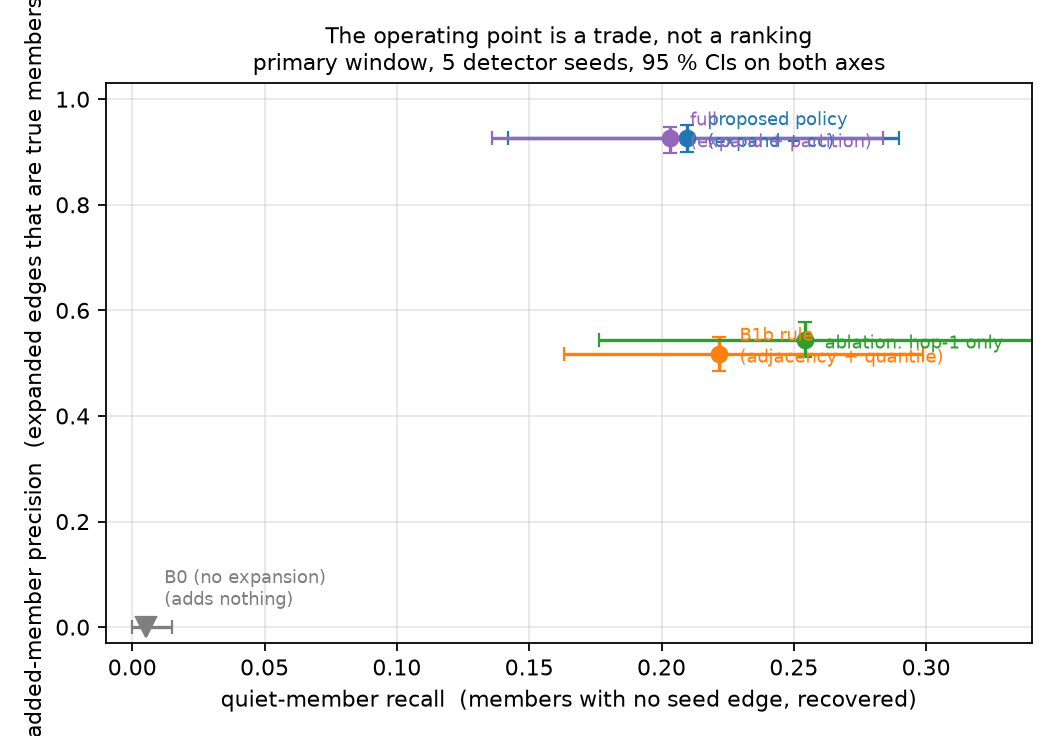
\includegraphics[width=0.55\textwidth]{r9_quiet_vs_precision.png}
\caption{Quiet-member recall against added-member precision (day-folded policy inputs, as first
reported; with leak-free inputs the policy's added-member precision is 0.819). The rule and the
policy recover similar shares of quiet members; they differ in how many wrong edges they add.}
% source: results/figures/r9_quiet_vs_precision.png (repository figure)
\label{fig:quiet-precision}
\end{figure}


\subsection{Community detection is not a stronger baseline than components}
\label{sec:results-baselines}

Replacing connected components with community detection on the same flagged-edge graph does
not help (Table~\ref{tab:ring-methods}, upper block; edge weight is the larger detector score
between two accounts, and the seed fraction is chosen on validation per seed). The best
community method by validation ring-F1, Louvain at resolution 0.5, reaches 0.515 on test,
against 0.521 for seeds and connected components ($-0.006$ [$-0.014$, $+0.000$],
$p_{\mathrm{Holm}}=0.072$) and 0.589 for the full pipeline ($-0.074$ [$-0.118$, $-0.035$],
$p_{\mathrm{Holm}}=0.0004$). Higher resolutions split rings apart (Louvain at resolution 2:
0.107). On the learned policy's expanded subgraph, label propagation in place of components
gives 0.555, below both components (0.582) and the average-linkage partition (0.589). CSGM,
collaborative scatter-gather mining~\citep{tian2025}, is designed for one pattern family and
uses no detector; over five random two-institution splits it reaches 0.083, with ring recall
0.048 over all eight pattern types. These comparisons were added after the main results.
% source: results/tables/v40_external_baselines.json (bar_B: louvain_r0.5 best by val; compare vs b0 / full, paired unit bootstrap 10,000 draws, Holm over two); v45_posthoc_ring_ci.csv (test_visible rows); results/notes/p3_baselines.md

\paragraph{An account-flagging method converted to rings.}
TAML~\citep{rico2026} flags illicit accounts per day and explains each with a signature. We trained it
on our split with its published settings (three seeds), took accounts above a validation-chosen
threshold on the two test days, and formed rings as connected pieces of its own graphs restricted
to those accounts. It reaches ring-F1 \ci{0.327}{0.254}{0.403} (precision 0.379, recall 0.287); a
per-day conversion gives 0.323. Three labels apply. Its features aggregate all ten days, test days
included; about 42\,\% of in-window ring transactions are absent from its graphs (247 of 585); and
so at most 63 of the 97 matchable rings can be formed. On those 63 its recall is 0.788. TAML solves
account flagging; converted to rings, it loses mainly through what its graphs omit. An exploratory
paired comparison with seeds-only MEGA-GenAgg rings ($+0.224$ [$+0.146$, $+0.304$]) is not a
superiority test.
% source: results/notes/p9_taml.md (2026-11-18 section); results/notes/final_numbers.md (TAML); experiments/R15_taml/scored_3seed_10k, paired_genagg_b0_vs_taml_joined

\subsection{Partition: not significant at 174 rings, resolved at 2{,}187}
\label{sec:results-partition}

On HI-Small the partition stage is not significant ($+0.015$ matched rate
[$-0.002$, $+0.036$], $p_{\mathrm{Holm}}=0.49$), nor is partitioning without expansion
($p_{\mathrm{Holm}}=0.23$). On HI-Medium, with 2{,}187 rings, an effect of the same size is
resolved: $+0.015$ [$+0.010$, $+0.020$], $p_{\mathrm{Holm}}=0.0003$
(Section~\ref{sec:results-hm}).
% source: results/tables/v3_closeout_p3.csv (global, full vs b2: mean_delta 0.01486, lo 0.00983, hi 0.01989, p_holm 0.0003)
Its pre-registered hypothesis --- that partitioning would allow a
looser seed budget --- was rejected: validation ring-F1 falls from 0.593 to 0.194 as the seed
fraction grows from 0.10\,\% to 0.50\,\%. A Louvain partition of the same expanded subgraph
leaves ring-F1 unchanged at 0.582.
% source: r9_significance.csv (full_vs_b2, cc_partition_vs_b0); docs/FINDINGS.md (B3, B4); results/tables/r4_partition.csv (b4)
On MEGA-GNN scores, where merged rings are commoner, the gain is the same size ($+0.017$)
and its interval excludes zero ($p_{\mathrm{Holm}} \approx 0.011$): over-merged rings fall
from 9.8 to 8.2 per seed there and stay at 5.2 on ours. The stage removes over-merges only
where they exist, and pays for recall with precision on both detectors.
% source: docs/FINDINGS.md (B3)
Its apparent benefit also depends on two evaluation choices: the recall gain is $+0.024$ at
Jaccard 0.3, $+0.015$ at 0.5 and $+0.001$ at 0.7, and it reverses when only connected pieces
of three or more accounts are scored (Section~\ref{sec:findings-scope}), on both releases.
On HI-Small we do not claim the partition step beyond neutral. Typing, held-out pattern types and time-to-detection are
in the released repository.
% source: docs/FINDINGS.md (B3; dated note, component-level scope)

\subsection{Transfer to a larger release}
\label{sec:results-hm}

On HI-Medium (test days 6--14, 2{,}187 rings), a detector trained only on HI-Small and applied
without retraining gives seeds-only ring-F1 $0.396 \pm 0.015$ over five seeds, against 0.090 for
an earlier HI-Medium-trained detector that differs in architecture and training data and has two
usable seeds (Table~\ref{tab:hm-transfer}; Section~\ref{sec:findings-saturation}). Paired over
the 2{,}187 rings the difference is $+0.306$ [$+0.286$, $+0.326$]; it comes from precision as
much as recall. We do not read this as transfer beating in-domain training: the comparison
changes the detector and its training data at once.
% source: results/notes/final_numbers.md (HI-Medium transfer); results/tables/hm_transfer_paired_addendum5.csv
Most of the gain is ranking, not budget allocation. The earlier detector put most of its global
budget on one day; allocating seeds per day lifts it to 0.148, while the transferred detector
stays at 0.387, so allocation explains at most about 0.06 of the 0.24 gap that remains.
% source: final_numbers.md (jump decomposition, five seeds); experiments_hi_medium/closeout_a15/log_seed{1,2}.json
The expansion policy and the partition were trained on HI-Medium with the earlier detector and
lack two of their inputs under transfer, so they are not evaluated here. With the earlier
detector, the release's 2{,}187 rings do resolve effects that 174 cannot: the partition gain is
$+0.015$ [$+0.010$, $+0.020$] (Section~\ref{sec:results-partition}).
% source: results/tables/v3_closeout_p3.csv (global, full vs b2)

% Source: results/notes/final_numbers.md (HI-Medium transfer section); results/tables/hm_transfer_closeout_seed{1..5}_ci.csv;
% results/tables/hm_transfer_paired_addendum5.csv (paired unit bootstrap over 2,187 rings, 10,000 draws, seeds averaged per draw).
\begin{table}[t]
\centering
\caption{Seeds-only rings (B0) on HI-Medium, test days 6--14, 2{,}187 rings, global 0.1\,\% budget,
in-window members, Jaccard $\ge 0.5$. The two detectors differ in architecture and training data.}
\label{tab:hm-transfer}
\small
\begin{tabular}{lcccc}
\toprule
Detector (seeds) & Precision & Recall & Ring F1 & Ring F1, per-day budget \
\midrule
Trained on HI-Small only, no retraining (5) & 0.444 & 0.357 & $0.396 \pm 0.015$ & $0.387 \pm 0.015$ \
Trained on HI-Medium, earlier detector (2) & 0.126 & 0.074 & 0.090 & 0.148 \
Paired difference & $+0.318$ & $+0.283$ & $+0.306$ [$0.286$, $0.326$] & -- \
\bottomrule
\end{tabular}
\end{table}


\subsection{Edge F1 is not a proxy for ring recovery}
\label{sec:results-swap}

We re-ran the ring layer on other detectors at the same fixed 0.1\,\% seed budget, re-choosing
every other downstream parameter on validation per detector and seed (Figure~\ref{fig:edge-ring}, Table~\ref{tab:detector-swap}).
Our MEGA-GNN reproduction reaches $0.6856 \pm 0.0447$ test edge F1, against the
$0.7083 \pm 0.0218$ its authors report for the same configuration; the gap is attributable to
batch-causal sampling (Section~\ref{sec:data}), which their setup does not use\footnote{All MEGA-GNN scores in this paper are produced with a scoring batch of 2048 transactions. The released models were originally scored at 8192, which gives test edge F1 $0.6893 \pm 0.0396$ against $0.6856 \pm 0.0447$ at 2048; per seed, 2048 minus 8192 is $-0.0126$, $-0.0029$, $-0.0013$, $+0.0049$ and $-0.0069$. The causal neighbour sampler cuts batches by size or by 30 minutes of seed time, whichever comes first, so a larger scoring batch lets a transaction see later transactions of the same batch (median look-ahead 180\,s at 2048, 600\,s at 8192). The validation-to-test gap per seed is in the released repository.}.
% source: results/notes/p7_genagg.md (batch-2048 per-seed table, look-ahead); results/notes/p7_batch_span.json
% source: docs/paper/generalisation.md §1

\begin{figure}[t]
\centering
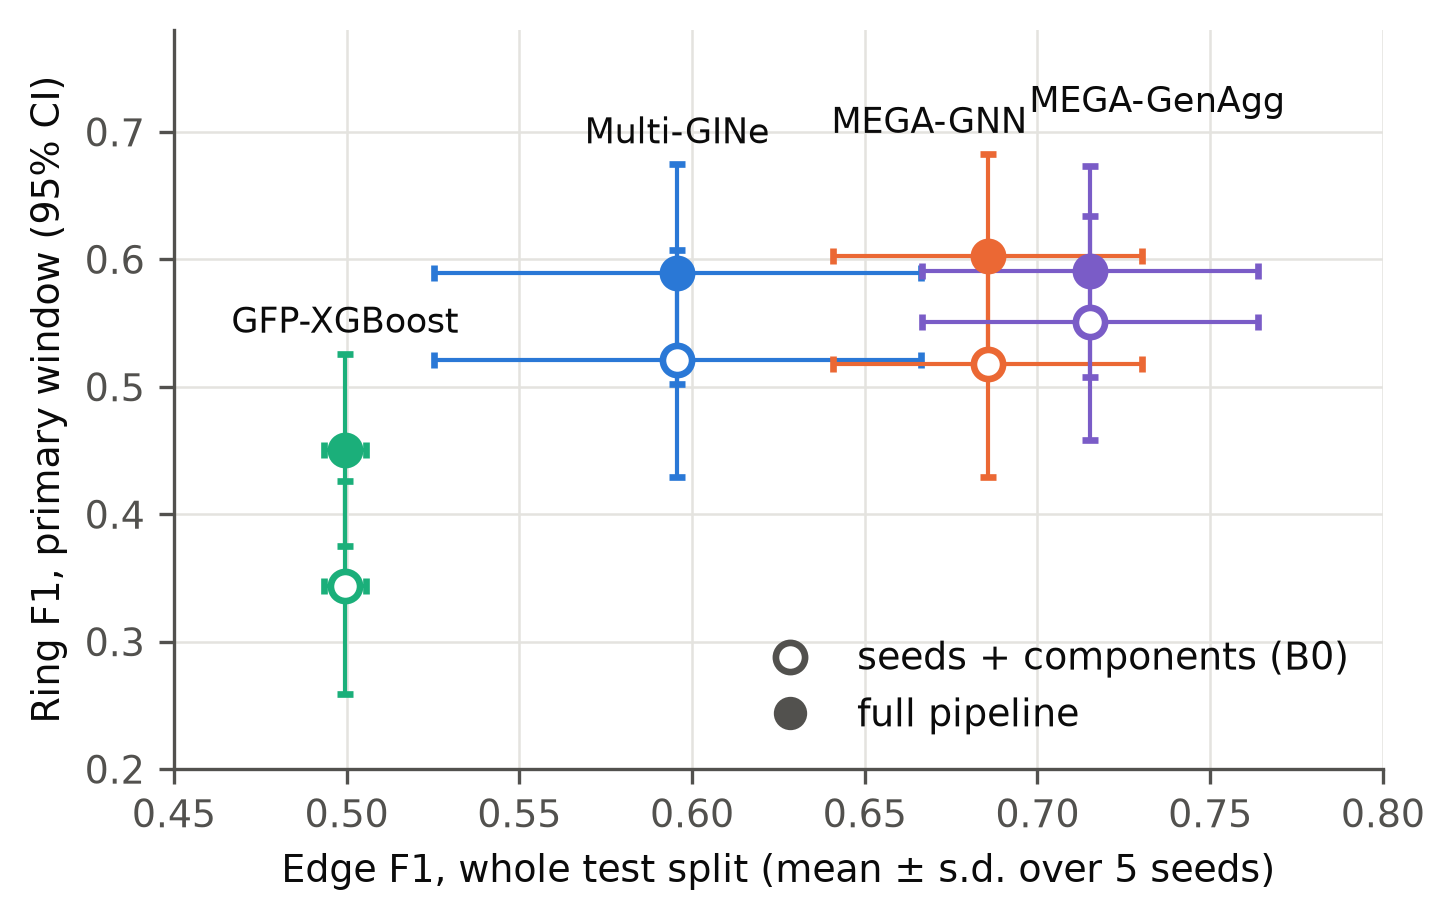
\includegraphics[width=0.62\textwidth]{fig_edge_vs_ring_sb2048.png}
\caption{Edge F1 against ring F1 for four detectors (scoring batch 2048). From Multi-GINe to
MEGA-GenAgg, 12 points of edge F1 leave seeds-only ring F1 within 0.03; below Multi-GINe, ring
F1 falls with edge F1.}
% source: results/tables/r6_detector_swap_sb2048.csv, r6_genagg_5seed.csv; figure built by evaluation/make_figs_sb2048.py
\label{fig:edge-ring}
\end{figure}

% Source: results/tables/r6_detector_swap.csv
\begin{table}[t]
\centering
\caption{The same ring layer on three detectors, every downstream parameter
re-chosen on validation per detector per seed. Edge F1 is on the whole test split (mean $\pm$
std over 5 seeds); ring numbers are on the primary window with bootstrap CIs. Added-member precision here was measured with day-folded expansion-policy inputs; with leak-free (ring-folded) inputs the reference full pipeline's value is 0.817 (Table~\ref{tab:precision-paired}).}
% source (leak-free value): results/tables/v45_ringfold_full_precision_paired.csv (full_ringfold, added_member_precision 0.8174)
\label{tab:detector-swap}
\small
\begin{tabular}{lccccc}
\toprule
Detector & Edge F1 & Ring F1, B0 & Ring F1, full & Quiet rec., full & Added prec., full \\
\midrule
GFP-XGBoost & $0.500 \pm 0.006$ & \ci{0.343}{0.259}{0.426} & \ci{0.451}{0.375}{0.526} & 0.267 & 0.260 \\ % source: r6_detector_swap.csv (gfpxgb rows)
Multi-GINe (shipped) & $0.596 \pm 0.071$ & \ci{0.521}{0.429}{0.607} & \ci{0.589}{0.502}{0.675} & 0.203 & 0.926 \\ % source: r6_detector_swap.csv (gine_causal rows)
MEGA-GNN & $0.689 \pm 0.040$ & \ci{0.521}{0.432}{0.609} & \ci{0.607}{0.521}{0.688} & 0.242 & 0.932 \\ % source: r6_detector_swap.csv (mega rows)
\bottomrule
\end{tabular}
\end{table}


MEGA-GNN outscores Multi-GINe by 9.0 points of edge F1 and produces the same baseline rings
(ring-F1 0.518 vs.\ 0.521) at the fixed budget. MEGA-GenAgg, 12.0 points above Multi-GINe
($0.715 \pm 0.049$), gives seeds-only ring-F1 0.551, a paired difference of $+0.030$
[$-0.011$, $+0.072$]; with the full pipeline the difference is $+0.002$ [$-0.030$, $+0.034$].
% source: results/notes/final_numbers.md (detector-swap rows); results/tables/r6_genagg_paired.csv (exploratory family, Holm over 4) When validation chooses the budget instead,
two MEGA-GNN seeds pick 0.05\,\% and its rings fall behind (Section~\ref{sec:method}).
% source: results/tables/r6_detector_swap_sb2048.csv; docs/FINDINGS.md (C6)
This is not the detectors agreeing. MEGA-GNN's and Multi-GINe's seed sets overlap at Jaccard
0.409, yet they reach 127.4 and 129.6 of the 174 truth rings. What binds at this operating point is how many rings a
0.1\,\% quantile can reach, not the ranking that fills it. The relation is a ceiling, not
independence: the weaker GFP-XGBoost, 9.6 edge points below, loses 17.7 ring points.
% source: docs/FINDINGS.md (C6)
The claim is conditional on this budget, these graph neural detectors (edge F1 0.60 to 0.72)
and this dataset; below that range the detector still decides recovery
(Section~\ref{sec:results-hm}).
% source: results/tables/r6_seed_overlap_sb2048.csv

\paragraph{Can the budget be spent better?}
Each GNN detector touches about 74\,\% of truth rings and their touched sets overlap at
70.6\,\%, so their union reaches 150.8 of 174 --- but that is two full budgets. At the same
budget, a best-rank ensemble of the two reaches 133.6, about a fifth of the gap, because 484
of the 864 selected edges are in both detectors' top 0.1\,\%. A per-account budget reaches
fewer (116.2). At an equal budget neither reallocation changes baseline ring-F1 beyond seed
noise (0.521 / 0.515 / 0.519), and under the full pipeline the ensemble's gain
($+0.021 \pm 0.038$) is inside seed spread.
% source: docs/FINDINGS.md (C7, B14 with its dated correction); results/tables/v37_realloc_full.csv

\paragraph{The effective test budget is about half the nominal one.}
Only 463 of 864 seeds land in the primary window (Section~\ref{sec:findings-tail}). Spending the
whole budget inside it reaches more rings (148.2 against 129.6) but lowers ring-F1 from 0.589 to
0.546 on every seed, so the reported ring-F1 is not depressed by the budget lost to the tail
(table in the released repository).
% source: results/tables/v34_window_budget.json; docs/deep-analysis.md §1

\section{Where ring recovery stops}
\label{sec:results-ceiling}

Figure~\ref{fig:decomposition} accounts for all 174 truth rings. With the full pipeline on
Multi-GINe, the detector we use for loss counts throughout, 80.2 are matched per seed, 48.6 have fewer than three visible members and
go unmatched, 33.2 are untouched by any seed or expanded edge, 5.2 are merged with a
neighbour and 6.8 are recovered only in part. Achieved ring recall is
\ci{0.461}{0.393}{0.529}.
% source: docs/FINDINGS.md (B11); results/tables/r6_detector_swap.csv; r9_ring_ci.csv (average, primary, ring_recall)

\begin{figure}[t]
\centering
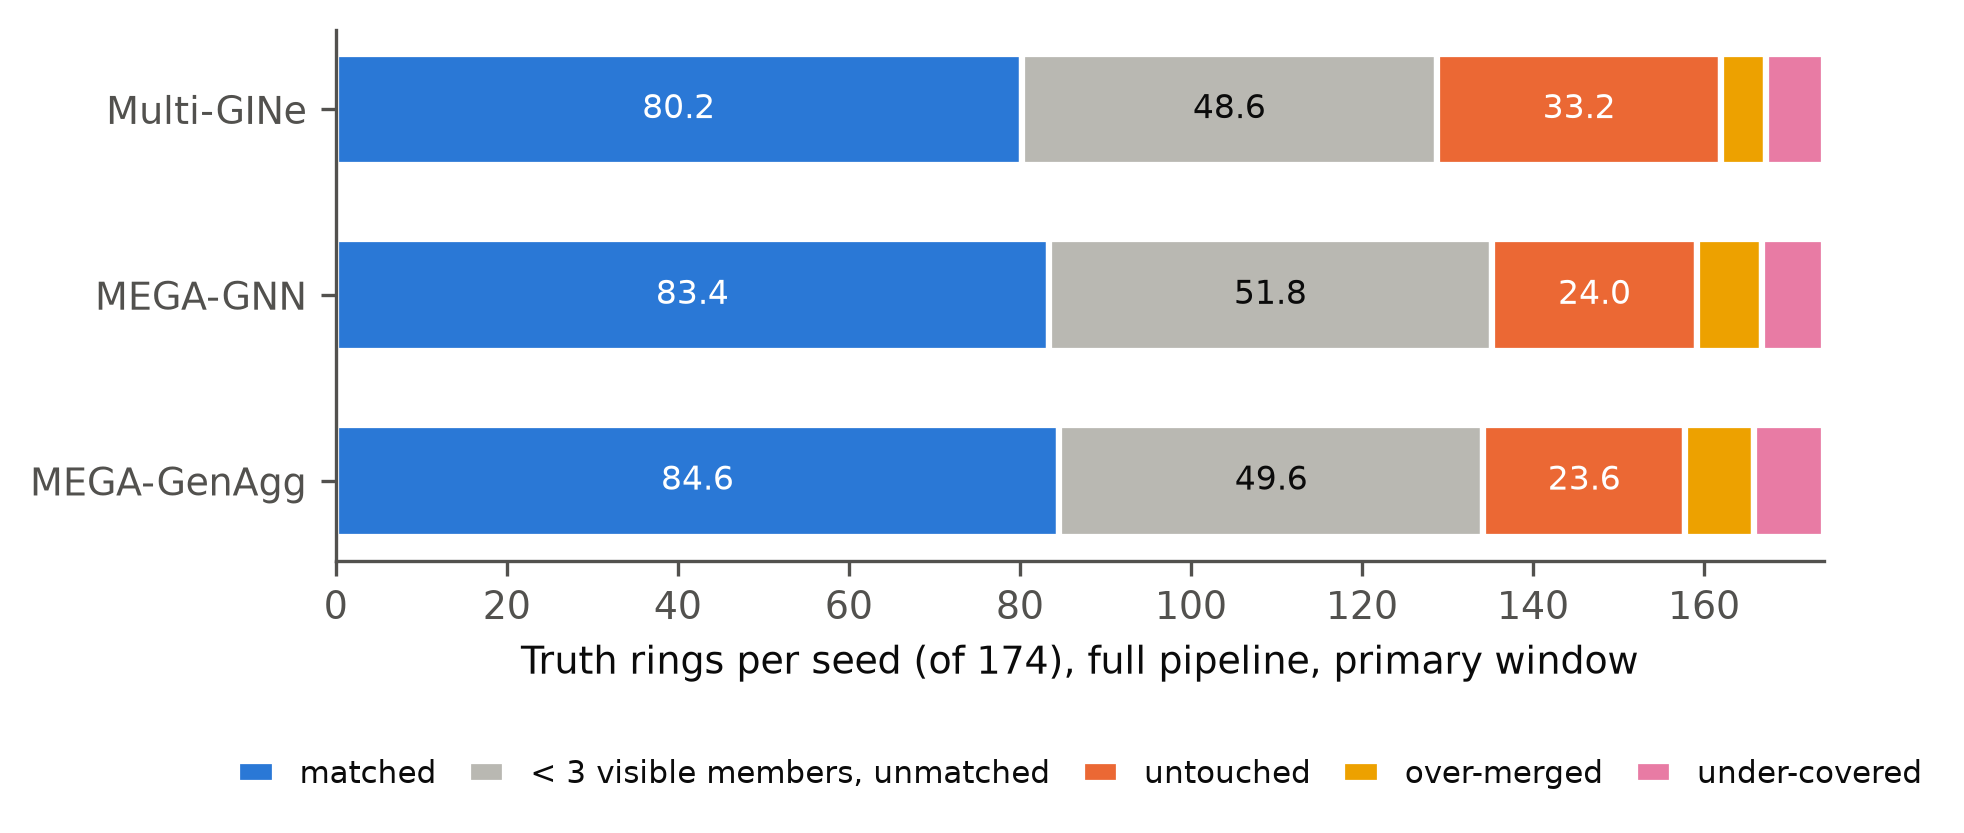
\includegraphics[width=0.9\textwidth]{fig_ring_decomposition_sb2048.png}
\caption{What happens to the 174 primary-window truth rings (per seed, full pipeline). The text
uses the Multi-GINe bars; the other detectors are shown for comparison only.}
% source: docs/FINDINGS.md (B11); figure built by paper_draft/make_figs.py
\label{fig:decomposition}
\end{figure}

\paragraph{Small rings are not a hard ceiling.}
60 of the 174 rings have fewer than three visible members, yet the pipeline matches
$11.4 \pm 2.3$ of them per seed, most at Jaccard 1.0, because \texttt{min\_size} applies to
the unrestricted prediction while matching uses the window-restricted one. The share of rings
with three or more visible members (114 of 174) is a reference level, not a bound.
% source: docs/FINDINGS.md (B7, B9, as corrected)

\paragraph{Partially recovered rings are clean, short fragments of long patterns.}
In every one of the 34 partially recovered instances the prediction contains no wrong
account, and it holds a median 3 of the ring's 14 members. Thirteen distinct rings produce all
34 instances, half of them STACK.
% source: docs/FINDINGS.md (B12); results/tables/r_under_covered.csv

\paragraph{Most of what is missing is disconnected inside the window.}
For each partially recovered ring we measured the distance from the recovered fragment to the
ring's missing member edges, through the ring itself, inside the primary window. 176 of 216
missing edges (81.5\,\%) lie in a piece with no path to the fragment at all --- all 140 for
STACK, all 24 for BIPARTITE --- and 85.6\,\% were never generated as candidates. The exception
is GATHER-SCATTER, whose 31 missing edges sit one hop away and were declined by the policy; an
oracle admitting exactly those edges completes all 8 instances, about 1.6 rings per seed,
whereas lowering the policy's floor to reach them costs more precision than validation
accepts.
% source: docs/FINDINGS.md (B13, B15); results/tables/r_in_window_connectivity.csv
Widening the window to all ten test days reduces disconnection to 52.3\,\% and removes it for
CYCLE and RANDOM, but STACK stays at 100\,\% (237 of 237): its chains are severed by the
train/validation/test split itself. Traversing the full 18-day graph backwards under the
expansion's own rules reaches none of the 140 missing STACK edges at two or three hops, and a
permutation null reaches none of 216.
% source: docs/FINDINGS.md (B13, B16); results/tables/r_historical_bridge.csv
A supervised-contrastive head~\citep{khosla2020} trained on the frozen detector embeddings to
recognise ring identity does not reconnect the pieces either: same-ring separability across
components rises only from AUC 0.552 to 0.618, against a bar of 0.75 fixed in advance.
% source: docs/deep-analysis.md §10 — registered follow-up; not yet recorded in docs/FINDINGS.md

\paragraph{Observability, counted directly.}
77 of the 174 rings (44\,\%) have no connected in-window piece of three or more accounts. 60
of them are the small rings above; the other 17 have enough visible members, split across
pieces that are each too small, and are scored as ordinary misses. On the 97 rings that do
have a matchable piece, the pipeline recovers 70.6\,\% of the pieces, and STACK recall rises
from 0.036 to 0.493.
% source: docs/FINDINGS.md (dated note, component-level scope); results/tables/v36_component_scope.csv

Taken together, the binding constraint is neither seed allocation nor policy thresholds. It is
how much of a ring is observable and connected inside the evaluation window --- a property of
the split and the scope rule that is easy to mistake for a property of the method.

\subsection{What did not help}
\label{sec:results-negative}
We made nine attempts to spend the seed budget better or to reassemble rings after the
detector, all at the fixed 0.1\,\% budget (primary window, test-visible truth, Jaccard 0.5, five
seeds, Multi-GINe scores): five were read on test and four stopped at their validation gate. None
raised ring-F1. The reference is the shipped full pipeline, or for the verifier, motif search and
flow-following the leak-free one; both score 0.589 on test.
% source: results/notes/recovery_attempts.md (list confirmed against q_track, m_track, recovery_ensemble, recovery_history, FINDINGS B14)
\begin{itemize}
\item \emph{Best-rank seed fusion} of two detectors (test): $+0.021 \pm 0.038$, inside seed spread.
\item \emph{Per-account seed budget} (test): fewer rings reached (116.2 against 129.6) and lower ring-F1.
% source: docs/FINDINGS.md (B14); results/tables/v37_realloc_full.csv
\item \emph{Account-level seeding} (test): $-0.138$ [$-0.184$, $-0.093$].
% source: results/notes/q_track.md (Q2); results/tables/q_family_holm.csv
\item \emph{Over-generate at 0.2\,\% and verify} (test): $+0.004$ [$-0.041$, $+0.046$]; precision up
$0.098$, recall down $0.029$.
% source: results/tables/m1_primary.json
\item \emph{History-reserved seeds} for accounts with labelled history (test): $+0.003$ [$-0.022$, $+0.030$].
% source: results/notes/recovery_history.md (B2); results/tables/b2_test_r25_both_paired.csv
\item \emph{Undersized-group rescue} (validation): no relaxed cell beat the shipped one.
% source: results/notes/q_track.md (Q6)
\item \emph{Temporal motif search} and \emph{flow-following} (validation): both gates failed (0.569 against 0.585).
% source: results/tables/m2_gate.json, m3_gate.json
\item \emph{Rank-averaged detector ensemble} as the seed source (validation): 0.575 against 0.593.
% source: results/notes/recovery_ensemble.md
\end{itemize}
The loss breakdown says why (Multi-GINe full pipeline, per seed; the one detector we use for loss
buckets throughout). Of 174 rings, 77 have no in-window piece of three or more accounts (11.4 of
them still matched), 11.0 are matchable but touched by no seed, 14.4 are recovered too thinly, and
merges (1.0) and splits (1.8) account for little; 68.8 are matched. Of the 93.8 unmatched rings,
65.6 are in the first group. Reassembly can only rearrange what the seeds already reach.
% source: results/notes/q_track.md (Q0 table); results/tables/q0_buckets.csv
